% Project report for the prediction system (stages S22-S33). Same format as main.tex (the earlier five-question study, which is kept unchanged).
% Every number is copied from reports/project/tables/*.csv (file named in each caption) or from reports/project/RESULTS_REGISTER.md; none is computed here.
% Compile on Overleaf with pdfLaTeX + biber. Upload this file, project_ref.bib, images/unilogo.png and the folder reports/project/figures (see \graphicspath).
\documentclass[12pt]{report}

\usepackage[T1]{fontenc}
\usepackage[utf8]{inputenc}
\usepackage{mathptmx}
\usepackage{float}
\usepackage{graphicx}
\graphicspath{{images/}{../project/figures/}{./}}
\usepackage{amsmath,amssymb,amsfonts}
\usepackage{textcomp}
\usepackage[table]{xcolor}
\usepackage[hidelinks]{hyperref}
\usepackage{url}
\usepackage{ragged2e}
\usepackage{array,multirow,booktabs}
\usepackage{biblatex}
\ExecuteBibliographyOptions{sorting=none}
\addbibresource{project_ref.bib}

\usepackage[parfill]{parskip}
\usepackage{geometry}
\usepackage{sectsty}
\chapterfont{\centering}
\geometry{paper=a4paper, top=1in, bottom=1in, left=1.2in, right=0.8in, headheight=0.75cm, footskip=1.5cm, headsep=0.75cm}
\linespread{1.5}
\newcommand{\unexpl}{\emph{not explained by measured cost drivers}}

\begin{document}
\begin{titlepage}
	\centering
	\begin{figure}[htbp]\centering
\includegraphics[height=4cm,width=4cm]{unilogo.png}\end{figure}
	\vspace{1cm}
	{\huge\bfseries Comilla University \par}
	\vspace{0.5cm}
	{\scshape\Large\bfseries Bangladesh Food Price Watch: A Price Forecasting and Abnormal-Rise Alert System for Dhaka Retail Food Prices\par}
	\vspace{0.45cm}
	{\scshape\Large\bfseries A RESEARCH PROJECT REPORT \par}
	{\scshape\Large\bfseries \textit{Submitted By}\par}
	{\Large\textbf{ROMJAN CHOWDHURY}}\par
	{\Large{Roll No.: 22408024}}\par
	\vspace{0.35cm}
	{\large\textbf{\textit{In Partial Fulfillment for the course Research Project of}}}\par
	{\Large\textbf{MASTER OF SCIENCE\\}}
	\vspace{0.1cm}
	{\large\textbf{IN }}
	{\large\textbf{DEPARTMENT OF COMPUTER SCIENCE AND ENGINEERING}\par}
	\vspace{0.45cm}
	{\Large\textbf{COMILLA UNIVERSITY, CUMILLA-3506}}\par
	\vspace{0.35cm}
	{\Large\bfseries November 2026}\par
\end{titlepage}

\newpage
\begin{center}
    \large\textbf{BONAFIDE CERTIFICATE}\\
\end{center}
\pagenumbering{gobble}
\section*{}
This is to certify that this research project entitled \textbf{``Bangladesh Food Price Watch: A Price Forecasting and Abnormal-Rise Alert System for Dhaka Retail Food Prices''} is submitted by Romjan Chowdhury, Roll No. 22408024, in partial fulfillment of the requirements for the degree of Master of Science in Computer Science and Engineering, Comilla University, Cumilla, and was carried out under my supervision. This is the bonafide work.
\\
\\
\begin{table}[h]
\begin{tabular}{l@{\hspace{3cm}}l}
{Signature} & {Signature} \\
\\
\ldots\ldots\ldots\ldots\ldots\ldots\ldots\ldots\ldots & \ldots\ldots\ldots\ldots\ldots\ldots\ldots\ldots\ldots \\
{Dr. Mahmudul Hasan} & {Dr. Mahmudul Hasan} \\
\textbf{Chairman of the Exam Committee} & \textbf{Supervisor} \\
{Associate Professor} & {Associate Professor} \\
{Department of CSE} & {Department of CSE} \\
{Comilla University, Cumilla.} & {Comilla University, Cumilla.} \\
\end{tabular}
\end{table}

\pagenumbering{Roman}

\chapter*{Abstract}%
\addcontentsline{toc}{chapter}{\numberline{}Abstract}%
This project builds a working price watch for the daily retail prices that the Trading Corporation of Bangladesh (TCB) publishes for Dhaka. From 63 items observed over 1,412 report days (May 2021 to October 2026), one LightGBM model forecasts 54 long-history items 1, 7, 14 and 30 report days ahead, gives each forecast an expected range built from the item's own recent errors, flags a price that stays above that range on 3 of the last 5 report days, and splits each alert into the parts attributed to price history, calendar, weather, the Indian onion export measures and the exchange rate. Every setting was fixed on calendar 2024 and written down before the test period (January 2025 to October 2026) was scored once. The forecasts did not beat ``tomorrow equals today'': relative error was 1.010, 1.001, 1.001 and 1.001 at the four horizons, and the model was statistically worse at 1 and 7 report days (Diebold--Mariano $p=0.0001$ and $0.011$). The alert rule, set at the 0.95 level from 2024 false alarms, detected 7 of 12 documented price episodes (11 of 16 product rows), but random dates reached a recall of 0.59 (placebo $p=0.26$), and only 6\% of alert runs started inside an event window. Driver shares changed a lot between refits, so the breakdown is only a rough guide. The pipeline, exports and a dashboard are working, but with these data the forecasts add little to persistence and the alerts are not yet reliable enough to act on.

\chapter*{Acknowledgement}
\addcontentsline{toc}{chapter}{\numberline{}Acknowledgements}
First and foremost, I would like to thank the Almighty Allah for His blessings that enabled me to complete this work.

\noindent I would like to express my sincerest thanks to my supervisor \textbf{Dr. Mahmudul Hasan}, Associate Professor, Department of Computer Science and Engineering, Comilla University, for his guidance on this research project, ``Bangladesh Food Price Watch''.

\noindent I would also like to acknowledge the Trading Corporation of Bangladesh, whose published daily price reports are the source of the price data, and the providers of the open driver data used here: Open-Meteo, the Federal Reserve Bank of St.\ Louis and the market data services behind the exchange-rate series.

\noindent Finally, I express my gratitude to my family and friends for their constant encouragement and support.

\newpage
\renewcommand*\contentsname{Table of Contents}
\tableofcontents

\listoffigures
\listoftables
\pagenumbering{arabic}

\chapter{Introduction}

\justifying

\section{Background}
Rice, edible oil, sugar, onion, eggs and lentils take a large share of what a Bangladeshi household spends on food, so a sudden rise in any of them is noticed quickly and often becomes a policy question. The Trading Corporation of Bangladesh (TCB) publishes a retail price report for Dhaka on most working days. The reports are Excel sheets with a minimum and maximum price per item, and they are not available as one clean, machine-readable series. Published forecasting work on Bangladeshi retail prices is thin and mostly uses price history alone \cite{agripricebd}.

The TCB prices have a shape that makes forecasting harder than it first looks. A price stays exactly the same on most days and then moves in a step. For administered items such as sugar and edible oil the step follows an announcement. For perishables such as onion and eggs the steps are smaller and more frequent. The median item had an unchanged price on 85 to 93 percent of report days, depending on its group (Table~\ref{tab:strata}). A forecast of ``no change'' is therefore right most of the time, and any model has to beat that to be worth running.

\section{What this project builds}
The aim was a system, not a comparison of methods. For each TCB item the system should do four things: forecast the price at 1, 7, 14 and 30 report days ahead; attach an expected range to the forecast; raise an alert when the price stays above that range; and say how the alert splits across the cost drivers that could be measured. The system should also run end to end from the raw price file to an export that a person can look at, and it should be possible to add new report days later and run it again.

A few rules were fixed before any results existed. One model is used for all items and all horizons, and other models appear only in the model-selection step. All choices of model, settings and alert threshold are made on calendar 2024 data. The test period, January 2025 to October 2026, is scored once, after the settings are written to a file and committed. If the model does not beat ``tomorrow equals today'', the report says so. A rise that the measured drivers do not account for is called \unexpl, and nothing in the report claims to know its cause. The alerts detect abnormal rises after they have started; they are not an early warning.

\section{Report organization}
Chapter 2 gives the related work in brief. Chapter 3 describes the data, the model, the validation design and the alert rule. Chapter 4 reports the results in the order the system produces them, then discusses limitations. Chapter 5 concludes.

\chapter{Related Work}
Most published work on forecasting retail food prices compares a handful of models on a few items. For Bangladesh, a recent benchmark of classical and deep models on a new market price dataset is the closest study I found, and it reports forecasts from price history only \cite{agripricebd}. The systems side, meaning ranges, alerts and an explanation of each alert, is less often reported than the accuracy numbers.

On the method side I use standard tools. Exponential-smoothing models are chosen automatically with the information-criterion search of Hyndman and Khandakar's family of methods, which is what the ETS candidate in Chapter 4 does. LightGBM is a gradient-boosted tree learner that handles mixed numeric inputs and missing values without much preparation \cite{lightgbm}, and its hyper-parameters were searched with Optuna \cite{optuna}. For scoring, I follow the advice to report a scale-free error and a ratio to a naive benchmark \cite{hk2006}. Differences between two forecasts are tested with the Diebold--Mariano test and its small-sample correction \cite{dm1995,hln1997}. Whether the share of prices above an upper bound matches its nominal rate is checked with the proportion-of-failures test of Kupiec \cite{kupiec}. The driver breakdown uses the additive per-feature contributions of a tree model, the quantity that SHAP reports for trees \cite{shap}, summed over groups of features. Work on onion price transmission in Bangladesh \cite{onionnardl} is the reason the Indian onion export measures are among the drivers.

\chapter{Data and Method}

\section{Price data}
The price file holds 76,440 rows: 63 items observed over 1,412 report days from 17 May 2021 to 24 October 2026. Nine of the items started to be reported only in May 2024 and have too little history to forecast, so the model covers the other 54. Table~\ref{tab:strata} lists the groups used in the evaluation. A price of zero or a blank cell means the item was not reported that day; such cells are never filled in a forecast target.

Reporting was irregular in 2022. Only 24 reports exist between 12 March and 31 December 2022. That period is never filled, never used as a target and never scored, and any input window that touches it is dropped from training.

I checked the file against the original Excel sheets with a machine re-read of a random 2\% sample: 1,530 item-day rows on 28 report days and 3,060 price cells. No row or cell differed, which puts the transcription error rate below 0.25\% (Wilson 95\% upper limit, Table~\ref{tab:audit}). This audit only checks copying. It cannot show that TCB itself typed a value correctly.

\begin{table}[H]\centering\small
\caption{Items by evaluation group. Source: reports/project/tables/P2\_panel\_summary.csv.}\label{tab:strata}
\begin{tabular}{lrrr}
\toprule
Group & Items & Report days & Median share of days with unchanged price \\
\midrule
Imported staples & 19 & 1,412 & 0.932 \\
Volatile perishables & 10 & 1,412 & 0.874 \\
Spices & 8 & 1,412 & 0.892 \\
Administered & 7 & 1,412 & 0.848 \\
Domestic staples & 7 & 1,412 & 0.906 \\
Non-food & 3 & 1,412 & 0.918 \\
Short history (not forecast) & 9 & 591 & 0.928 \\
\bottomrule
\end{tabular}
\end{table}

\begin{table}[H]\centering\small
\caption{Audit of the price file against the original TCB sheets. Source: reports/project/tables/P2\_audit\_summary.csv.}\label{tab:audit}
\begin{tabular}{lr}
\toprule
Measure & Value \\
\midrule
Rows sampled and checked & 1,530 \\
Report days in the sample & 28 \\
Price cells checked (minimum and maximum) & 3,060 \\
Cells that differ & 0 \\
Cell error rate, Wilson 95\% upper limit & 0.00125 \\
Row error rate, Wilson 95\% upper limit & 0.0025 \\
\bottomrule
\end{tabular}
\end{table}

\section{Drivers}
Four outside series are joined to the prices, each on the date it would have been known. Weather comes from Open-Meteo for 13 locations, with a five-day publication lag; the three features kept are the 7-day maximum temperature, the 30-day mean temperature and the 7-day rainfall, and they are mapped to seven items. The exchange rate is the Bangladeshi taka per US dollar, taken as the last value on or before the report day, as a level and a 30-day change, and it is mapped to 34 items (imported staples, administered items and spices). The onion export measure is a flag that is 1 while an Indian duty, minimum export price or ban on onions is in force, for the two onion items. The calendar features are the month, the day of the week, the days to Ramadan and to the two Eids, a Ramadan flag, holidays in the coming week and the days since the previous report. A driver that is missing stays missing, with a flag, and is never set to zero. A daily driver older than seven days is dropped rather than carried further.

The table of exporter events ends on 27 March 2025, so the onion flag is empty for every report day after that, which covers most of the test period.

\section{Targets, inputs and the single model}
For each item and report day $t$, the target at horizon $h \in \{1,7,14,30\}$ is the change in log price between $t$ and $t+h$ report days, defined only if the price at $t+h$ was actually reported. The input price is the last reported price, carried forward, because TCB sometimes skips a report for an item. The price-history inputs are the log price, log changes over 1, 7, 14 and 30 report days, the deviation of the price from its 30-report mean, the 30-report volatility of one-day changes, and the number of reports since the price last changed.

One LightGBM model is fitted on rows of all four horizons stacked together, with the horizon as an input. A forecast is the last price times the exponential of the predicted change. The model sees only rows whose target date lies on or before the forecast origin, so nothing from the future enters training. Table~\ref{tab:features} lists the 25 inputs by group.

\begin{table}[H]\centering\small
\caption{Model inputs by driver group. Source: reports/project/tables/P3\_driver\_inventory.csv and config/project.yaml.}\label{tab:features}
\begin{tabular}{p{3.2cm}p{7.8cm}p{2.4cm}}
\toprule
Group & Inputs & Items with a value \\
\midrule
Price history & log price, log changes, deviation from rolling mean, rolling volatility, reports since change, item and group codes, horizon & all 54 \\
Calendar & month, weekday, days to Ramadan and each Eid, Ramadan flag, holiday in next 7 days, days since previous report & all 54 \\
Weather & 7-day maximum temperature, 30-day mean temperature, 7-day rainfall & 7 \\
Onion export measure & 1 while an Indian onion export duty, price floor or ban is in force & 2 \\
Exchange rate & log taka per dollar, 30-day change & 34 \\
\bottomrule
\end{tabular}
\end{table}

\section{Validation, selection and tuning}
Calendar 2024 is the validation year. Six candidates were compared on 43 forecast origins in 2024, spaced 7 report days apart: the naive forecast (no change), automatic ETS, ridge regression, a random forest, LightGBM and a small LSTM. The naive forecast is the yardstick and cannot be chosen. The primary score is the mean absolute error of the log price change, which is about the percentage error and does not depend on an item's price level. A simpler model is preferred if it is within 1\% of the best.

Tuning used Optuna with 50 trials, scored on origins from January to August 2024. The tuned setting was then compared with the default on origins from October to November 2024, and it was kept only if it was better there. The 2025--26 test period was not touched in either step.

\section{Test design}
Before the test was scored, the chosen settings, the 25 inputs, the list of metrics and the list of checks were written to a file and committed to the repository (state/prereg\_S27.yaml), and the code refuses to score the test unless that file is committed. The test has 87 forecast origins, again 7 report days apart, from January 2025 to October 2026, with the model refitted every 8 origins on all data up to the origin. Two further schemes check the main result: walk-forward on 2023 and 2024, and a sliding window of the latest 500 report days. The test was scored once. The 2025--26 period had already been scored by an earlier version of this study, so it is not a first look at that data.

The main metrics are the mean absolute error of the log change, the same error for the naive forecast, and their ratio per item. The ratio is summarised over items with a geometric mean, where 1 means a tie with ``tomorrow equals today'' and values above 1 mean the model is worse. I also report absolute error in taka, error on days where the price changed against days where it did not, direction accuracy on days the price moved, and the Diebold--Mariano test against the naive forecast.

\section{Ranges, alerts and the driver breakdown}
The expected range at horizon 7 comes from each item's own forecast errors. At a forecast origin, the item's last 120 errors whose target date had already passed are taken, and the 5th and 95th percentiles of those errors give the lower and upper bounds. An alert starts when the price is above the upper bound on at least 3 of the last 5 report days, and a run of consecutive alert days counts as one alert.

The alert level, that is which percentile to use, was chosen on 2024 data outside the windows of the documented price episodes: the lowest of 0.90, 0.95, 0.975 and 0.99 that gave at most 2 false alarms per item-year. That choice was committed (state/prereg\_S28.yaml) before any episode was scored. The 12 documented episodes come from news reports collected for the earlier study. An episode window runs from 14 days before the recorded onset to 30 days after the news peak, and an episode counts as detected if an alert starts inside the window for at least one affected item. The model is never trained on events and the level is never tuned on them.

For the breakdown, the model's per-feature contributions to a forecast are added up within each driver group, and the same sums are made for all items, for each item group and for each alert day. As a check on stability, three models fitted with data up to different report days (1011, 1211 and 1411) were compared on the same rows.

\section{Software and how it runs}
The code is in a public GitHub repository, and it contains no price data. Five Colab notebooks run the stages in order: data and features; model selection and tuning; the sealed test; alerts and drivers; and the production fit and export. Each stage writes its results to Google Drive and records a hash of every output, so a stage that has finished is skipped on a rerun. A sixth notebook shows the exports in a small Gradio app and downloads them. A local Streamlit dashboard reads the same three export files.

\chapter{Results and Discussion}

\section{Model selection on 2024}
No candidate beat the naive forecast on the 2024 validation origins (Table~\ref{tab:select}). ETS came closest, at 5\% worse than naive overall, LightGBM was 17\% worse, and ridge regression was worst. Because the naive forecast cannot be chosen, ETS was the nominal winner. The project's explanation step needs a tree model, so I kept LightGBM as the main model and logged that decision, together with this table, before tuning. This means the model was not chosen because it won the comparison, and the report should be read with that in mind.

\begin{table}[H]\centering\small
\caption{Validation on 2024, 43 origins, all four horizons. Lower is better; relative error 1.000 is a tie with ``tomorrow equals today''. Source: reports/project/tables/P5\_model\_selection\_overall.csv.}\label{tab:select}
\begin{tabular}{lrr}
\toprule
Model & Mean absolute error of log change & Relative to naive (geometric mean over items) \\
\midrule
Naive (tomorrow = today) & 0.0231 & 1.000 \\
ETS & 0.0235 & 1.053 \\
LightGBM & 0.0241 & 1.173 \\
LSTM & 0.0245 & 1.378 \\
Random forest & 0.0272 & 1.698 \\
Ridge regression & 0.0292 & 2.316 \\
\bottomrule
\end{tabular}
\end{table}

\section{Tuning}
Across the 50 trials the best score on the tuning origins was 0.02478 and the median trial was 0.02486, so most settings that were not clearly bad ended up almost the same. The default setting scored 0.02592 on the tuning origins and 0.02050 on the confirmation origins; the best trial scored 0.02478 and 0.01969. The tuned model is small: 6 leaves per tree, a learning rate of 0.0196, 400 trees, an L1 objective and fairly strong regularisation (L1 penalty 7.4, L2 penalty 2.0, a minimum of 76 rows per leaf). The tuning found a better setting, and it also found one that moves the forecast very little from zero.

\section{Test accuracy}
On the sealed test the model matches the naive forecast closely and does not beat it at any horizon (Table~\ref{tab:test}, Figure~\ref{fig:rel}). The geometric-mean relative error is 1.0096, 1.0013, 1.0009 and 1.0007 at horizons 1, 7, 14 and 30. At horizons 1 and 7 the model is worse by a margin that is small in size but clear in the Diebold--Mariano test ($p=0.0001$ and $0.011$); at horizons 14 and 30 there is no detectable difference ($p=0.92$ and $0.50$).

The reason is visible in the error split. Most of the error comes from days when the price moved: at horizon 7 the error is 0.0467 on days the price changed and 0.0001 on days it did not, and the price changed on 26\% of those forecasts. The model predicts almost no change, so it is nearly perfect on unchanged days and about as wrong as the naive forecast on changed ones. $R^2$ on the price changes is between $-0.002$ and $0.012$. Direction is right on only 15\% to 38\% of the days where the price moved, which is what a forecast of no change would give. The learning curve agrees: over 400 trees the training error went from 0.0305 to 0.0302 and the error on a holdout of the latest 15\% of report days did not improve (0.0171 to 0.0172, Figure~\ref{fig:lc}). Adding trees gave the model nothing more to learn from these inputs.

\begin{table}[H]\centering\small
\caption{Sealed test, January 2025 to October 2026, 87 origins. Relative error is the geometric mean over 54 items of model error divided by naive error. Sources: reports/project/tables/P7\_accuracy\_by\_horizon.csv and P7\_dm\_vs\_naive.csv.}\label{tab:test}
\begin{tabular}{rrrrrrr}
\toprule
Horizon & Model error & Naive error & Relative error & Error (Tk) & Price changed (share) & Diebold--Mariano $p$ \\
\midrule
1 & 0.0028 & 0.0027 & 1.0096 & 3.1 & 0.069 & 0.0001 \\
7 & 0.0120 & 0.0120 & 1.0013 & 23.8 & 0.256 & 0.011 \\
14 & 0.0199 & 0.0199 & 1.0009 & 43.2 & 0.377 & 0.92 \\
30 & 0.0323 & 0.0324 & 1.0007 & 79.2 & 0.524 & 0.50 \\
\bottomrule
\end{tabular}
\end{table}

\begin{figure}[H]\centering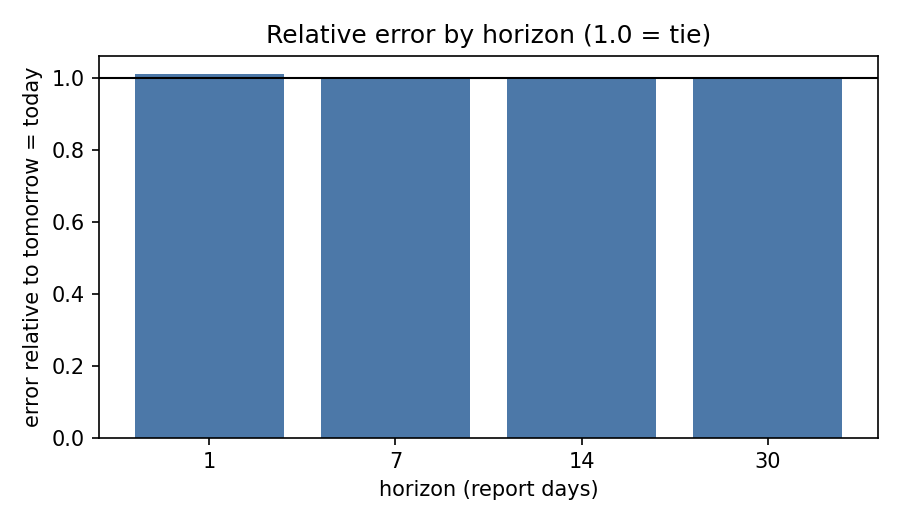
\includegraphics[width=0.7\textwidth]{F10_relative_error_by_horizon.png}\caption{Relative error by horizon on the test (1.0 is a tie with ``tomorrow equals today''). Source: reports/project/figures/F10.}\label{fig:rel}\end{figure}

Item by item the picture is the same. Out of 54 items, the model had a lower error than the naive forecast for 13 items at horizon 7, 13 at horizon 14 and 16 at horizon 30, and the ratio ranged from 0.96 to 1.03 (P7\_accuracy\_by\_item.csv). By group, the ratio was between 0.998 and 1.017 everywhere (Table~\ref{tab:group}). The only group-and-horizon cells below 1 are administered items at 30 days (0.999) and volatile perishables at 14 and 30 days (0.999 and 0.998), and these differences are far too small to count as evidence.

\begin{table}[H]\centering\small
\caption{Relative error to the naive forecast by item group and horizon on the test (geometric mean over items). Source: reports/project/tables/P7\_accuracy\_by\_group.csv.}\label{tab:group}
\begin{tabular}{lrrrr}
\toprule
Group & h = 1 & h = 7 & h = 14 & h = 30 \\
\midrule
Administered & 1.008 & 1.001 & 1.001 & 0.999 \\
Domestic staples & 1.017 & 1.004 & 1.002 & 1.002 \\
Imported staples & 1.003 & 1.001 & 1.001 & 1.002 \\
Non-food & 1.001 & 1.000 & 1.001 & 1.002 \\
Spices & 1.014 & 1.001 & 1.000 & 1.001 \\
Volatile perishables & 1.017 & 1.003 & 0.999 & 0.998 \\
\bottomrule
\end{tabular}
\end{table}

The two checks give the same answer, and the older walk-forward years are worse for the model (Table~\ref{tab:wf}). In 2023 the model was 11\% worse than naive at horizon 1 and 3\% worse at the other horizons. The sliding-window version was a little worse than the expanding window on the test. The error analysis (P7\_error\_analysis.csv) shows no difference between normal periods and the weeks around Ramadan and the Eids beyond a slightly larger error in the latter for both the model and the naive forecast (0.0126 against 0.0119 at horizon 7). The bias, meaning the mean of forecast minus actual in log terms, is close to zero (mean $-0.00008$ across origins at horizon 7, Figure~\ref{fig:bias}). The largest forecast errors are mostly for ginger in January 2025 at the 30-day horizon, with a log error of up to 1.4, and for potato and local onion at 30 days.

\begin{table}[H]\centering\small
\caption{Relative error to the naive forecast under the other evaluation schemes. Source: reports/project/tables/P7\_walk\_forward.csv.}\label{tab:wf}
\begin{tabular}{lrrrr}
\toprule
Scheme & h = 1 & h = 7 & h = 14 & h = 30 \\
\midrule
Rolling origin 2025--26 (main) & 1.0096 & 1.0013 & 1.0009 & 1.0007 \\
Walk-forward 2023 & 1.1143 & 1.0294 & 1.0272 & 1.0253 \\
Walk-forward 2024 (the tuning year) & 1.0343 & 1.0047 & 1.0027 & 1.0027 \\
Sliding window of 500 reports, 2025--26 & 1.0270 & 1.0078 & 1.0077 & 1.0047 \\
\bottomrule
\end{tabular}
\end{table}

\begin{figure}[H]\centering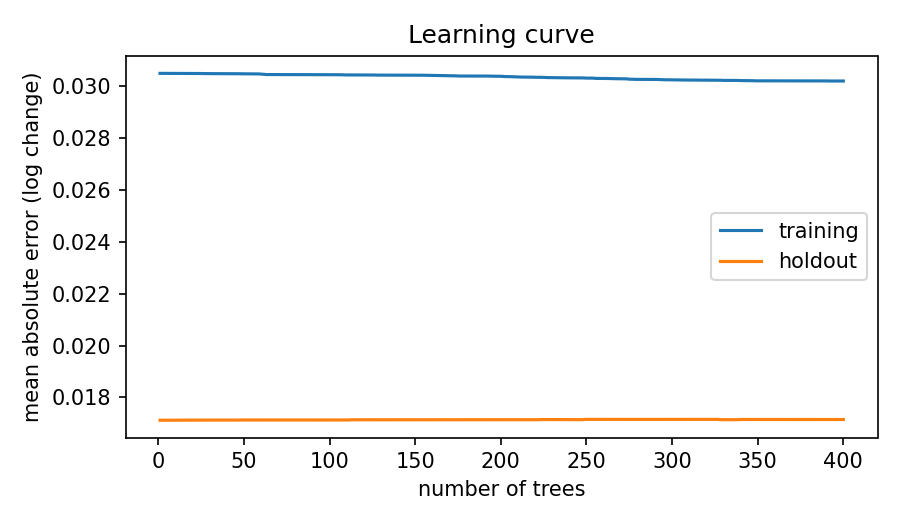
\includegraphics[width=0.7\textwidth]{F13_learning_curve.png}\caption{Training and holdout error by number of trees. Source: reports/project/figures/F13.}\label{fig:lc}\end{figure}

\begin{figure}[H]\centering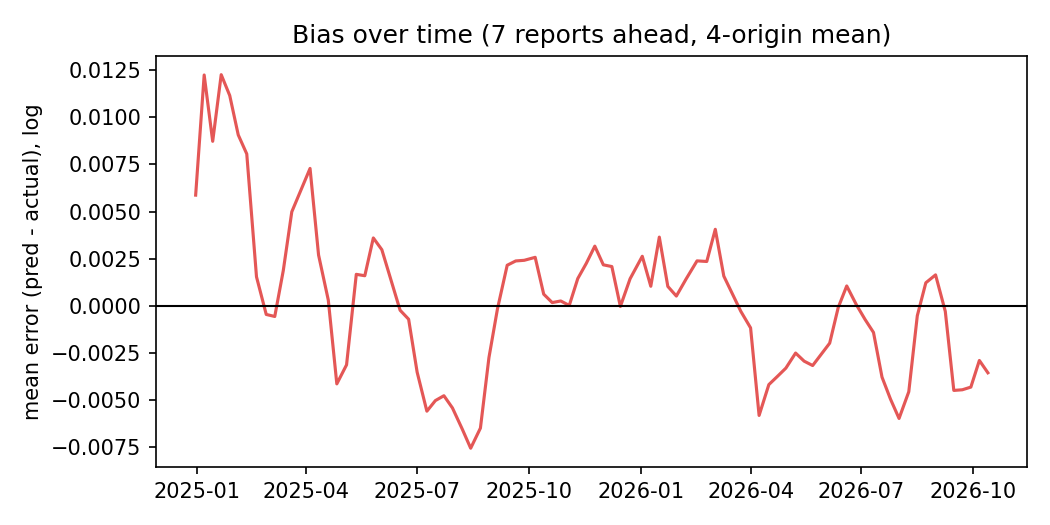
\includegraphics[width=0.75\textwidth]{F12_bias_over_time.png}\caption{Bias over time at horizon 7 (four-origin mean). Source: reports/project/figures/F12.}\label{fig:bias}\end{figure}

\begin{figure}[H]\centering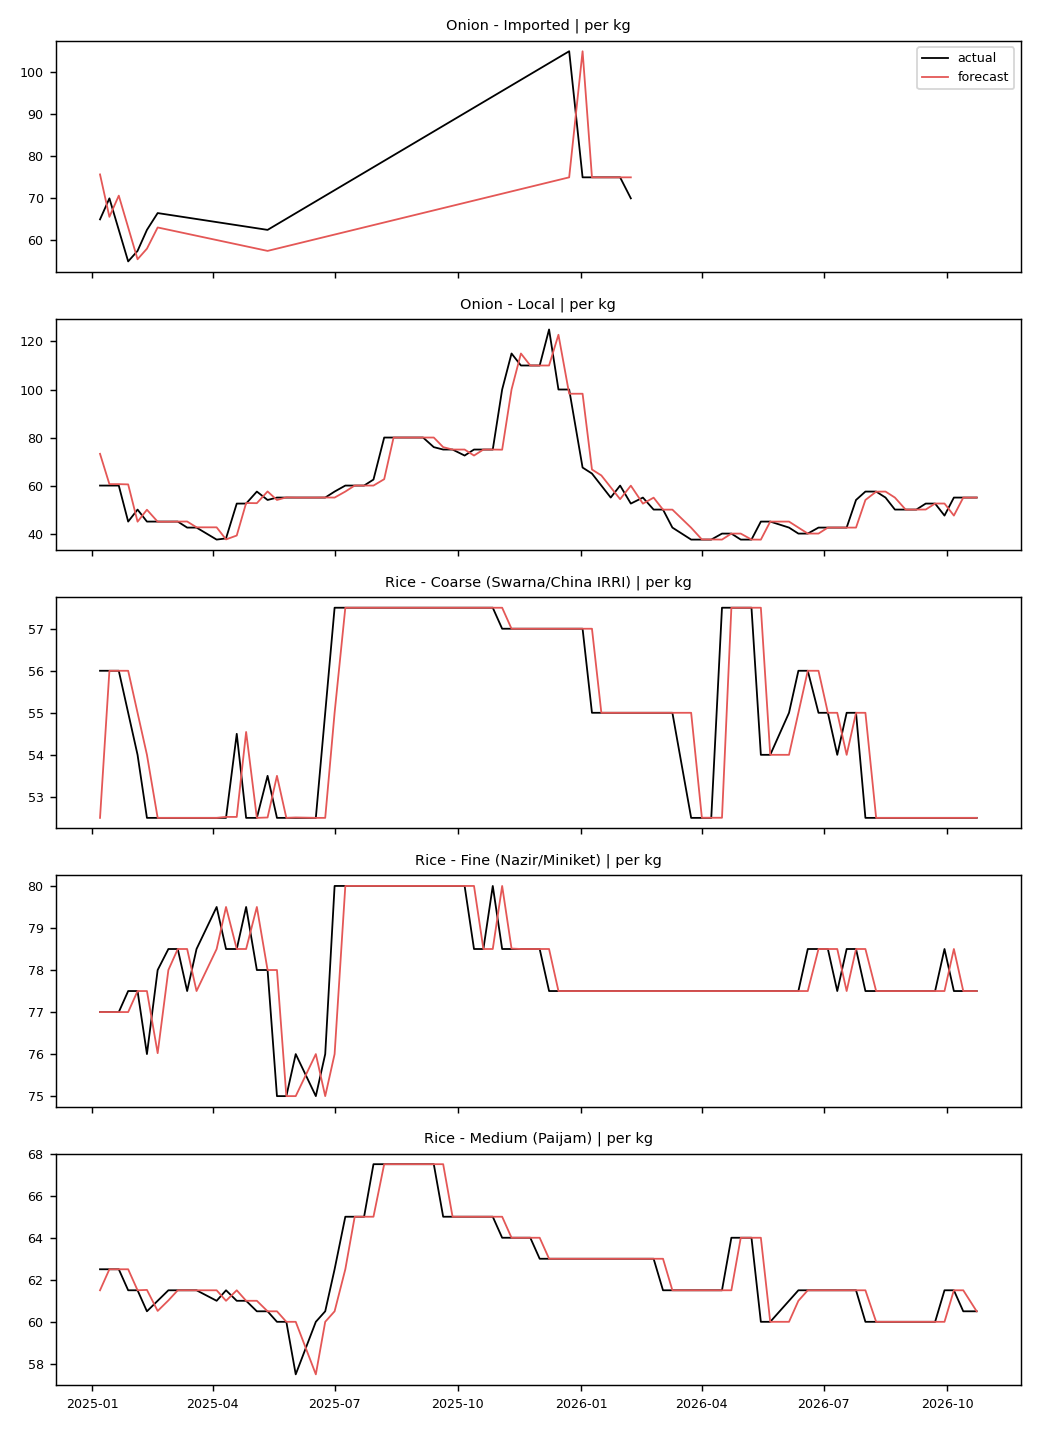
\includegraphics[width=0.85\textwidth]{F14_actual_vs_forecast.png}\caption{Actual and forecast prices at horizon 7 for five items on the test. The two lines are close because the forecast is almost always the last price. Source: reports/project/figures/F14.}\label{fig:avf}\end{figure}

\section{Expected ranges}
At horizon 7, over 55,337 daily forecasts from June 2023 to October 2026, the upper bound at the 0.95 level was exceeded on 5.9\% of days, against 5\% expected, so the upper bound covered 0.941 of the outcomes. The central interval between the 5th and 95th percentiles covered 0.883 against 0.90 expected. The Kupiec test rejects the nominal rate ($p<0.001$), but with this many dependent observations the test is strict, and the practical gap is under one percentage point on the upper side. The result was similar in the two periods (upper coverage 0.939 in 2023--24 and 0.943 in 2025--26), and the bound was narrower in the second period (mean width 0.088 against 0.121 in log terms). The ranges are slightly too tight, not badly so.

\section{Alerts}
Table~\ref{tab:level} shows how the alert level was chosen. At the 0.90 level there were 3.07 false alarms per item-year in 2024 outside the event windows, which is over the target of 2, and 0.95 was the lowest level under it (1.92). Level 0.95 was therefore fixed. The scoring of the episodes came after that.

\begin{table}[H]\centering\small
\caption{Alert levels. False alarms are alert runs per item-year in 2024 outside event windows; recall and precision are over the whole period, counted by product row. Source: reports/project/tables/P8\_level\_curve.csv.}\label{tab:level}
\begin{tabular}{rrrrr}
\toprule
Level & False alarms, 2024 & Event recall (product rows) & Precision & Alert runs \\
\midrule
0.90 & 3.07 & 0.688 & 0.061 & 635 \\
0.95 (chosen) & 1.92 & 0.688 & 0.061 & 429 \\
0.975 & 1.63 & 0.625 & 0.054 & 368 \\
0.99 & 1.44 & 0.500 & 0.052 & 327 \\
\bottomrule
\end{tabular}
\end{table}

At the chosen level, alerts started inside the window of 7 of the 12 episodes (11 of 16 product rows; Table~\ref{tab:events}). The misses are the sugar episode of June 2023, two potato episodes in 2024, the egg episode of October 2024 and the green chilli episode of July 2026. The negative lead times in the table should not be read as early warning. The windows open 14 days before the recorded onset and can run for months after the news peak (the rice episode runs to June 2025), so an alert that starts anywhere inside counts as a detection. The long windows also help the detection rate: a single alert run anywhere inside a 600-day window is enough.

The random-date control puts the detection rate in perspective. When each episode's window was moved to a random start inside the evaluation period, the mean recall was 0.59, against 0.69 observed, and 26\% of the random draws did as well or better ($p=0.26$ over 300 draws). So the alerts are not distinguishable from chance on these 12 episodes. Of 429 alert runs, only 6\% (26 runs) began inside an event window; the others were not matched to any of the documented episodes. Some of these may be real rises that were not in the news-based list, but the list is the only reference I have, and the system cannot tell the two cases apart.

\begin{table}[H]\centering\small
\caption{The 12 documented episodes and whether an alert started inside the window (level 0.95). Lead is the number of days between the first alert and the news peak, negative if before. Source: reports/project/tables/P8\_event\_scores.csv.}\label{tab:events}
\begin{tabular}{llllrl}
\toprule
Episode & Product & Onset & News peak & Detected & Lead (days) \\
\midrule
BD-S09 & Sugar & 2023-06-01 & 2023-06-25 & no & -- \\
BD-S11 & Eggs (farm) & 2023-08-01 & 2023-08-13 & yes & 0 \\
BD-S12 & Onion (imported, local) & 2023-08-01 & 2023-08-21 & yes & $-4$ \\
BD-S13 & Onion (imported, local) & 2023-10-01 & 2023-12-09 & yes & $-38$ \\
BD-S14 & Potato & 2023-10-01 & 2023-11-13 & yes & $-12$ \\
BD-S15 & Rice (coarse, medium) & 2023-10-01 & 2025-06-10 & yes & $-558$ \\
BD-S16 & Eggs (farm) & 2024-05-01 & 2024-05-19 & yes & $-11$ \\
BD-S17 & Potato & 2024-07-01 & 2024-08-18 & no & -- \\
BD-S19 & Potato & 2024-09-01 & 2024-09-05 & no & -- \\
BD-S20 & Eggs (farm) & 2024-10-01 & 2024-10-18 & no & -- \\
BD-S21 & Soybean oil (bottled, loose) & 2024-10-01 & 2025-02-09 & yes & $-125$ \\
BD-S22 & Green chilli & 2026-07-01 & 2026-07-31 & no & -- \\
\bottomrule
\end{tabular}
\end{table}

\section{Driver breakdown}
On the last 120 report days, price history accounts for 56\% of the average size of the model's contributions, the exchange rate for 17\%, the calendar for 14\%, the onion export measure for 10\% and weather for 4\% (Table~\ref{tab:drivers}). Because the model forecasts nearly zero change, these are shares of small numbers. They describe what the model leans on, not how much a driver moved a price. The shares look similar across item groups, with price history at 46\% to 68\% in every group, and the exchange rate larger for non-food items and spices (about 24\% and 22\%).

\begin{table}[H]\centering\small
\caption{Share of the average absolute contribution by driver group, last 120 report days. Source: reports/project/tables/P9\_driver\_overall.csv and P9\_driver\_stability.csv.}\label{tab:drivers}
\begin{tabular}{lrrrr}
\toprule
Group & Final model & Fitted to day 1211 & Fitted to day 1011 & Spread \\
\midrule
Price history & 0.556 & 0.359 & 0.241 & 0.315 \\
Exchange rate & 0.170 & 0.017 & 0.102 & 0.153 \\
Calendar & 0.138 & 0.009 & 0.122 & 0.130 \\
Onion export measure & 0.096 & 0.008 & 0.067 & 0.088 \\
Weather & 0.040 & 0.607 & 0.468 & 0.567 \\
\bottomrule
\end{tabular}
\end{table}

The breakdown is not stable. The model fitted to data up to report day 1211 gave weather 61\% and price history 36\%, and the model fitted to day 1011 gave weather 47\%. The final model gives weather 4\%. A tool that moves this much between refits cannot be used to say what drives a price, and I describe the drivers as helpful for specific items, not proven. Two sign checks were planned. The price-above-recent-mean input has the expected sign (correlation $-0.18$ with its contribution, meaning a price high against its recent mean pulls the forecast down). The exchange-rate check returned no value and I did not find out why in the time available. At horizons 1 and 7 the shares are identical to many decimals, which fits a model whose trees never split between those two horizons, in line with the finding that it forecasts almost no change.

For every alert day the export file lists the contribution of each group and the part of the rise above the upper bound, labelled \unexpl. The labelling is a statement about the model's inputs only. It does not say that anyone caused a rise.

\section{The system and its exports}
The production model is fitted on all report days up to 24 October 2026. The export holds 216 forecasts (54 items at four horizons), each with a lower and upper bound taken from the item's last 120 test errors at the 0.95 level, and the 429 alert runs. The ranges for horizon 1 are often narrow to the point of being a single number (for example the loose atta price of 50 Tk is forecast at exactly 50 Tk), which is a direct sign that the model mostly predicts no change. The dashboard shows the forecast and range for a chosen item, the recent alerts, and the driver chart for an alert day.

\section{Limitations}
The main limitation is the result itself: on these data the forecasts add nothing over persistence at any horizon, so the value of the system rests on its ranges, alerts and bookkeeping, and the alerts are weak. The model was also not selected on validation merit, as explained above, so a different choice might have done somewhat better, although the ETS result suggests not by much.

The test period was not a first look, because an earlier version of this study had scored it. The settings were fixed before this run, but that earlier exposure cannot be undone.

Twelve episodes is a small number, and five of them fall in 2024, the year used to set the level (the level was set from non-event days only, so the episodes did not influence it). With 12 episodes, a recall of 7 of 12 has a wide uncertainty band, and the placebo comparison has little power. The episode windows are long, which flatters detection, and the list of episodes may be missing real rises that would turn some of the 94\% of unmatched alert runs into correct ones.

The data have gaps. The 2022 reports are too sparse and are not used. The table of Indian onion export measures ends in March 2025, so the onion input is empty after that date. Weather and exchange-rate files end a few days before the end of the price file, which will matter when new reports are added. The audit covers copying only, and it was run on the extended price file whereas the model uses the file to 24 October 2026. TCB does not state terms for reusing its reports, so the price data and everything derived from it are kept out of the public repository, and the Gradio link of the dashboard is public while it runs.

Some things I did not do. I did not try to predict whether the price will change at all, separately from by how much, which the step-like prices suggest. I did not use market-level prices from WFP to say whether a rise is national or local, and I did not test a pretrained forecasting model such as Chronos-2 \cite{chronos2}. The driver breakdown has no independent check beyond the two sign tests.

\chapter{Conclusion}
This project delivered a price watch for TCB Dhaka retail prices that runs from the raw price file to forecasts, expected ranges, alerts and a driver breakdown, and the evidence says it is not yet useful for forecasting: on the 2025--26 test one LightGBM model was no better than ``tomorrow equals today'' at 1, 7, 14 or 30 report days, and slightly worse at the shortest two, because most TCB prices do not change on most days and the inputs I could measure did not predict the days when they do. The ranges came close to their nominal coverage and the alert rule, fixed on 2024 data, flagged 7 of 12 documented price episodes, but random dates did almost as well and about 94\% of alert runs were not tied to any documented episode, so the alerts should be read as a way to review unusual rises and not as a warning. The driver shares changed too much between refits to support claims about causes, and the fair summary is that the measured drivers were not shown to explain these prices. The most useful next steps are to model separately whether a price will change and by how much, to build a larger and independently checked list of price episodes, and to extend the onion export table beyond March 2025.

\begingroup
\let\clearpage\relax
\renewcommand{\bibname}{References}
\addcontentsline{toc}{chapter}{\numberline{}References}
\printbibliography
\endgroup

\end{document}
